\documentclass[11pt]{scrartcl}
\usepackage[utf8]{inputenc} % Kodierung der Textdatei mit Sonderzeichen
\usepackage[ngerman]{babel} % Sprache fuer Inhaltsverzeichnis etc.
\usepackage{amssymb} % Mathematische Symbole
\usepackage{amsmath} % Mehr mathematische Konstrukte
\usepackage{graphicx} % Um Bilder einbinden zu koennen
\usepackage{float} % fuer \begin{figure}[H]
\usepackage{icomma} % laesst das Komma als Dezimaltrennzeichen interpretieren
\usepackage[pdftex]{hyperref} % Hyperlinks im Dokument
\hypersetup{colorlinks=true, linkcolor=black, citecolor=black, filecolor=black, urlcolor=black, pdftitle={MHD-Generator - Projektpraktikum 09/10 Gruppe 5}}


\newcommand{\unit}[1]{\ensuremath{\,\mathrm{#1}}} % Einheiten schreiben sich immer aufrecht!
\newcommand{\degr}{\ensuremath{^\circ}}
\newcommand{\cel}{\ensuremath{\degr\mathrm{C}}}
\newcommand{\dif}{\ensuremath{\mathrm{d}}}
\newcommand{\pdif}[2]{\ensuremath{\frac{\partial#1}{\partial#2}}}
\newcommand{\ee}[1]{\ensuremath{\cdot 10^{#1}}}


\setlength{\parindent}{1em}
\setlength{\parskip}{0.5\baselineskip}


\title{MHD-Generator - Gruppe 5 WS 09/10, Projektpraktikum der Uni Erlangen}
\date{09.11.2009 -- 04.12.2009}
\author{Michele Collodo, Andreas Glossner, Karl-Christoph G\"odel, Bastian Hacker, Maria Obst, Alexander Wagner, David Winnekens}



\begin{document}
\sloppy % laesst Latex nicht ueber den Rand rausschreiben
\thispagestyle{empty}
\large{Projektpraktikum WS 09/10}
\hfill
\raisebox{-1.4cm}{
\includegraphics[width=5cm]{images/fau.pdf}}
\\[8\baselineskip]
\begin{center}
{\Huge\textbf{MHD-Generator}}
\\[2\baselineskip]
{\Large 09.11.2009 -- 04.12.2009}
\\[6\baselineskip]
{\huge\textbf{PPG 5}}\\[0.5\baselineskip]
{\large\textbf{
Michele Collodo,
Andreas Glossner,\\
Karl-Christoph G\"odel,
Bastian Hacker,\\
Maria Obst,
Alexander Wagner,
David Winnekens}\\
Tutor: Xiaoyue Jin}
\vfill



\small{\url{http://pp.physik.uni-erlangen.de/groups/ws0910/ppg5/ppg5\_start.html}}
\end{center}
\newpage



\tableofcontents
\vfill



\begin{abstract}
dumdidum
\end{abstract}
\newpage
%%%%%%%%%%%%%%%%%%%%%%%%%%%%%%%%%%%%%%%%%%%%%%%%%%
%Das Plexiglasteil wird im Folgenden: "Zelle" genannt
%%%%%%%%%%%%%%%%%%%%%%%%%%%%%%%%%%%%%%%%%%%%%%%%%%


\section{Einleitung}	%% maria: ist fertig, kommentare, wuensche, anregungen?
Die Frage der Energieerzeugung hat in der Physik der letzten Jahrhunderte immer eine bedeutende Rolle gespielt. Eine vielversprechende M\"oglichkeit schien das Ausnutzen von magnetischen Feldern. Die ersten \"Uberlegungen zu solchen Generatoren machte Michael Faraday schon 1832. Sp\"ater wurden immer mehr Arten entdeckt, Magnetfelder zur Stromerzeugung zu nutzen. Zur Anwendung kommen hier sowohl statische als auch ver\"anderliche Magnetfelder. Der wohl bekannteste MHD-Generator ist der Dynamo, der bis heute oft zur Energiegewinnung eingesetzt wird. Doch der Effekt l\"asst sich auch auf viel gr\"o\ss{}eren Skalen wiederfinden. So erzeugt zum Beispiel die Erde ihr sch\"utzendes Magnetfeld mit dem Dynamoprinzip. Auch f\"ur die Erzeugung und Beschleunigung stellarer Jets gibt es magnetohydrodynamische Modelle.

\section{Theorie}	%% maria

%%% mir faellt nix mehr ein, was koennt ich noch reinschreiben?

Das Prinzip des MHD-Generators beruht auf der Lorentzkraft,
\begin{equation*}
\vec{F} = q \cdot \left(\vec{v} \times \vec{B} \right),
\end{equation*}
die in einem Magnetfeld auf eine bewegte Ladung wirkt. Wird also eine leitende Fl\"ussigkeit durch ein m\"oglichst homogenes, starkes Magnetfeld geschickt, welches senkrecht zur Flussrichtung gerichtet ist, werden positive und negative Ladung entsprechend der Rechten-Hand-Regel in entgegengesetzte Richtungen abgelenkt. Bringt man dann in jeder dieser Richtungen je eine ELektrode an, kann man eine Spannung abgreifen und hat so eine Generatorzelle konstruiert. 

\section{Konstruktion und Aufbau}

\subsection{Konstruktion des Magnetfelds}		%%andi
Im Vorfeld der eigentlichen Messungen an der Zelle wurde die möglichst optimale Konstruktion des Magnetfelds ermittelt. Ziel war es bei einer Feldstärke von rund $0.1 T$ ein möglichst im gesamten Bereich der Zelle homogenes Feld zu erhalten.\
Zunächst wurden verschiedene Permanentmagneten eingesetzt, die jedoch allesamt unbefriedigende Ergebnisse lieferten. Die eingesetzten Stabmagneten erzielten eine maximale Feldstärke von $0.07T$, das der zur Verfügung stehenden Hufeisenmagneten war noch wesentlich niedriger. Die größte Feldstärke wurde an Ringpermanentmagneten ($B\approx0.3T$) gemessen; dieser Wert fiel jedoch schon im Abstand von wenigen $mm$ stark ab ($1/r^3$-Abhängigkeit) und war deshalb ebenfalls ungeeignet.\
Folglich wurde ein Aufbau mit Elektromagneten gewählt. Zum Einsatz kamen dabei vier Spulen mit je 1000 Windungen (Anordnung siehe \hyperref[bfeld-vor2]{Abb.~\ref{bfeld-vor2}}).

\begin{figure}[ht]
\begin{center}
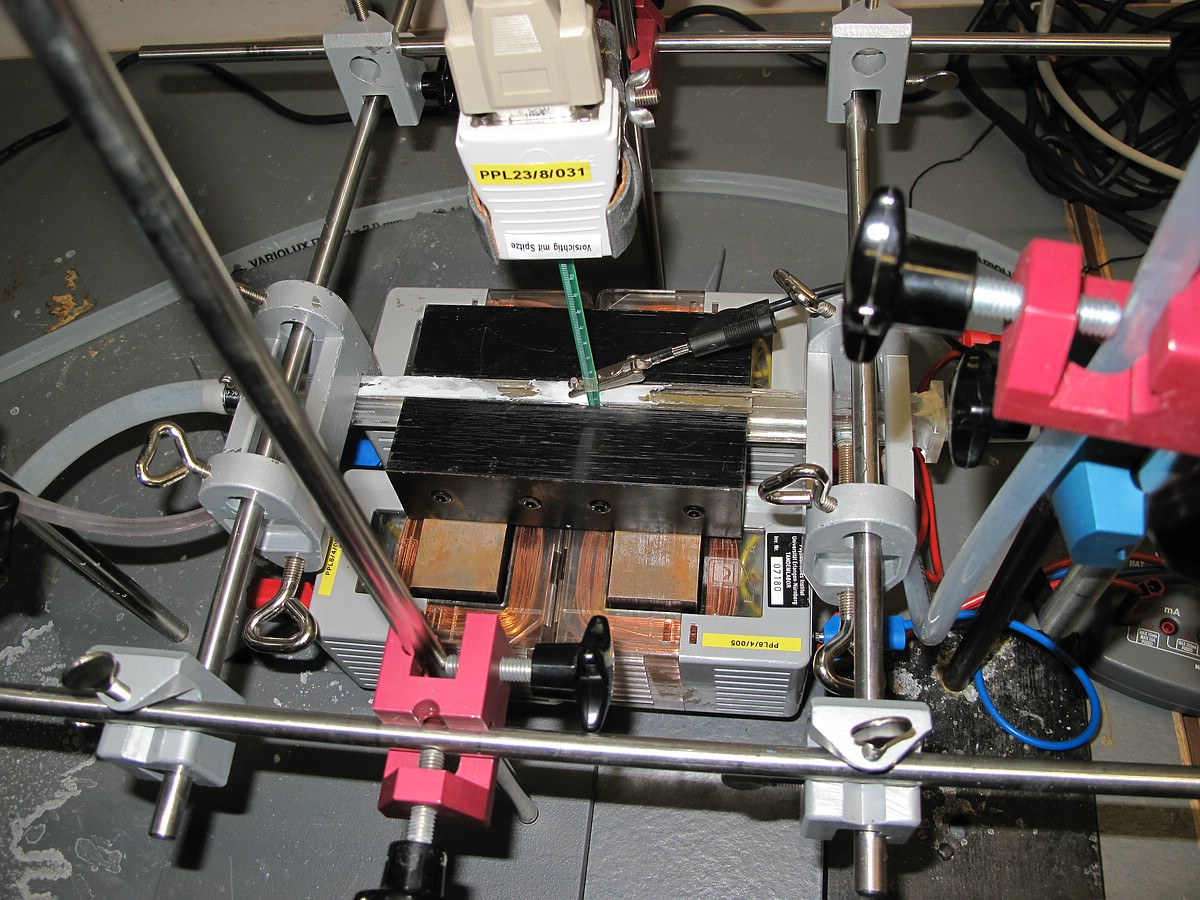
\includegraphics[width=0.8\textwidth]{images/bfeld-vor2.jpg}
\end{center}
\vspace{-1.5\baselineskip}
\caption{Anordnung der vier Spulen zum Erzeugen des Magnetfelds}
\label{bfeld-vor2}
\end{figure}

Zunächst wurde eine kurze Messung zur Ermittlung der Abhängigkeit der Magnetfeldstärke vom Abstand zwischen den beiden Eisenjochen
%% wie heissen die dinger schnell wieder
durchgeführt. Zu erwarten war wegen 
\begin{equation*}
B = \frac{\mu \cdot \mu_{0} \cdot N \cdot I}{\mu \cdot d + 2 \cdot \pi \cdot R}
\end{equation*}
in etwa eine $1/d$-Abhängigkeit, wobei $\mu$ die Materialkonstante des Eisens, $N$ die Windungszahl, $d$ der Abstand zwischen den beiden Eisenjochen und $R$ der Radius der "Gesamtspule" ist. Die "Gesamtspule" ist dabei die gesamte Anordnung der vier Einzelspulen und kann in erster Näherung als kreisförmig angenommen werden.
Permannentmageneten nicht geeignet, Vormessung B-Feld: Verschiedene Abstaende, Geometrie des Feldes, Schaltung der Spulenpaare

\begin{figure}[ht]
\begin{center}
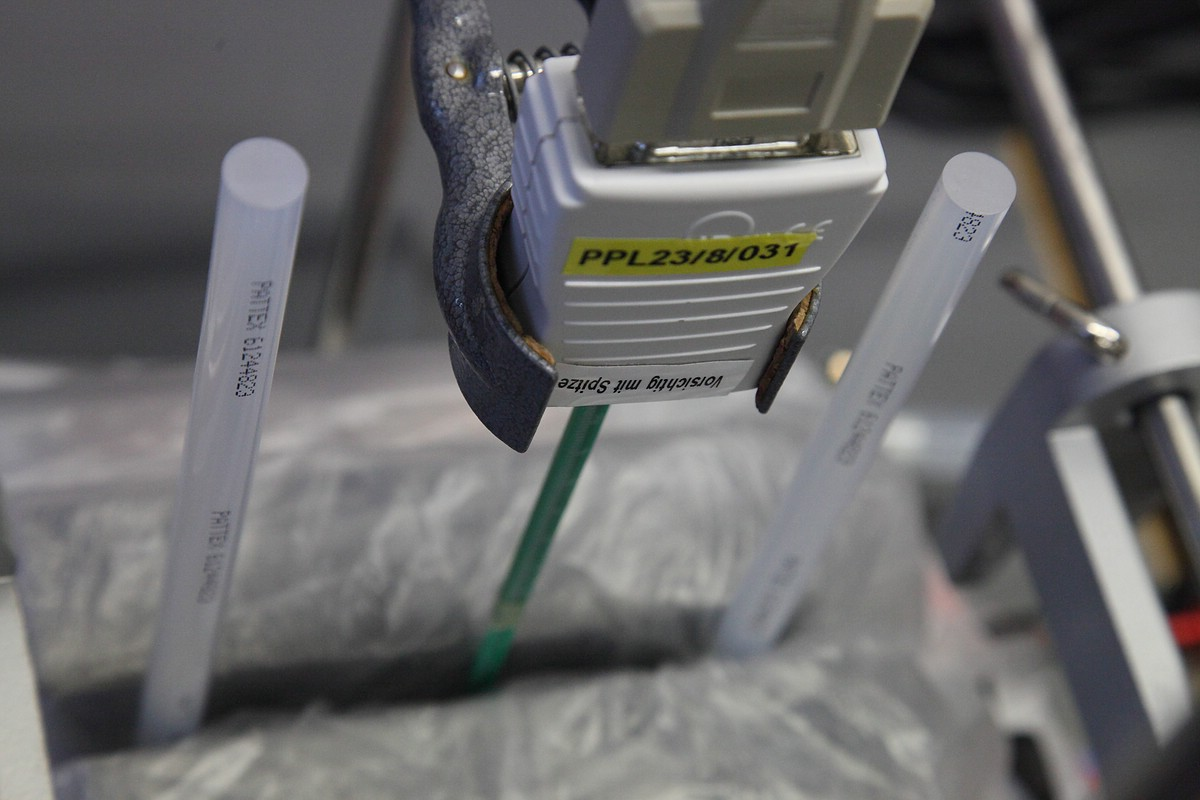
\includegraphics[width=0.8\textwidth]{images/bfeld-vor1.jpg}
\end{center}
\vspace{-1.5\baselineskip}
\caption{Vormessung ohne Zelle zur B-Feldst\"arke, die Plastikst\"abe dienen zum Einstellen verschiedener Spaltbreiten}
\label{bfeld-vor1}
\end{figure}

\subsection{Aufbau der Zelle}			%%karl
Platten, Anschl"usse, Abst"ande

\subsection{Aufbau der Messapperatur}		%% Axi
Nachdem die Zelle in der Werkstatt fertiggestellt worden war, wurde die restliche Versuchanordnung aufgebaut. Der MHD-Generator sollte folgende Komponenten enthalten:

\begin{itemize}
	\item Eine Pumpe mit einem Reservoir an ges\"attigtem Salzwasser 
	\item die Zelle, platziert in einem m\"oglichst homogenen Magnetfeld 	
	\item M\"oglichkeiten zur Messung der Magnetfeldst\"arke sowie des lokalen Drucks in der Zelle.
\end{itemize}

Die Pumpe wurde bereits im Vorraus im Versandhandel bestellt. Die ersten Vorabrechnungen hatten ergaben, dass eine Wassergeschwindigkeit im Bereich von $1m/s$ messbare Ergebnisse liefern w\"urde. Daher entschieden wir uns f\"ur eine Teichpumpe, die mit 220V Netzspannung betrieben wird und dabei laut Herstellerangaben bei einer Leistung von 16W ca. 1000l Wasser pro Stunde bis zu einer F\"orderh\"ohe von 1,7m transportieren soll. Da davon auszugehen war, dass diese nicht f\"ur den Einsatz in hoch konzentriertem Salzwasser geeignet ist, wurde der komplette Kreislauf am Ende jedes Arbeitstages mit Leitungswasser gesp\"ult um Langzeitsch\"aden vorzubeugen.

Beim Aufbau der gesamten Apperatur des MHD-Geneators musste mehreren Faktoren besondere Aufmerksamkeit geschenkt werden: 
\begin{itemize}
	\item Die Bereiche mit anliegenden Spannungen sollten getrennt von den wasserf\"uhrenden Bauteilen installiert werden. 
	\item Der Zelle muss waagrecht eingebaut sein, damit die Druckmessung nicht beeinflusst wird.
	\item Der Aufbau sollte genau reproduzierbar sein, um eine Vergleichbarkeit der Messungen zu erreichen.
	\item Bei einem Durchlauf sollten m\"oglichst viele Parameter gleichzeitig erfasst werden k\"onnen.
\end{itemize} 

\begin{figure}[ht]
\begin{center}
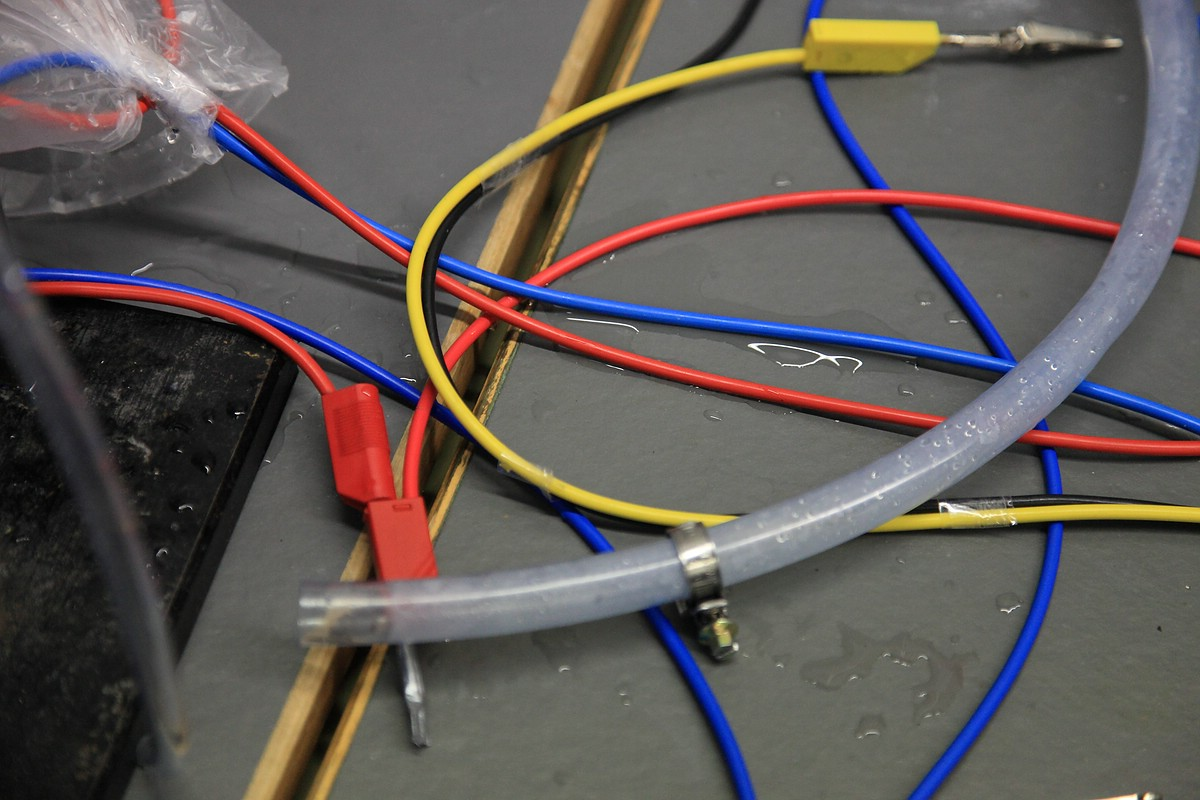
\includegraphics[width=0.8\textwidth]{images/wasser-strom1.jpg}
\end{center}
\vspace{-1.5\baselineskip}
\caption{Trennung der wasser- und stromf\"uhrenden Bereiche}
\label{wasser-strom1}
\end{figure}

Wie bereits beim ersten Projekt, erschien auch hier eine Konstruktion aus Stativstangen am Sinnvollsten. Die Zelle wurde an einem quadratischen Rahmen aus Stangen, Winkelverschraubungen, sowie Klemmen fixiert und konnte von oben in das Magnetfeld gesenkt werden. So war auch ein Umbau bei Bedarf relativ einfach m\"oglich. Eine vollst\"andige Trennung der strom- und wasserf\"uhrenden Teile ist aufgrund des MHD-Prinzips nicht m\"oglich. Daher befanden sich die Spulen und Eisenkerne mit den Stromanschl\"ussen in einer Plastikh\"ulle, die gen\"ugend Spielraum bot, um zwischen den Kernen die Zelle zu fixieren. 

Nachdem bei ersten Vormessungen entweder die Zelle oder die Magnetfeldsonde zwischen den  Spulen plaziert waren, entschieden wir uns auch die tangentiale B-Feld Sonde dauerhaft in den Kreislauf zu integrieren, um die Messwerte zusammenh\"angend aufzuzeichnen. Zwei d\"unne Abstandshalter stellten dabei sicher, dass die empfindliche Sonde nicht zwischen den Magneten zerdr\"uckt wird.

\begin{figure}[ht]
\begin{center}
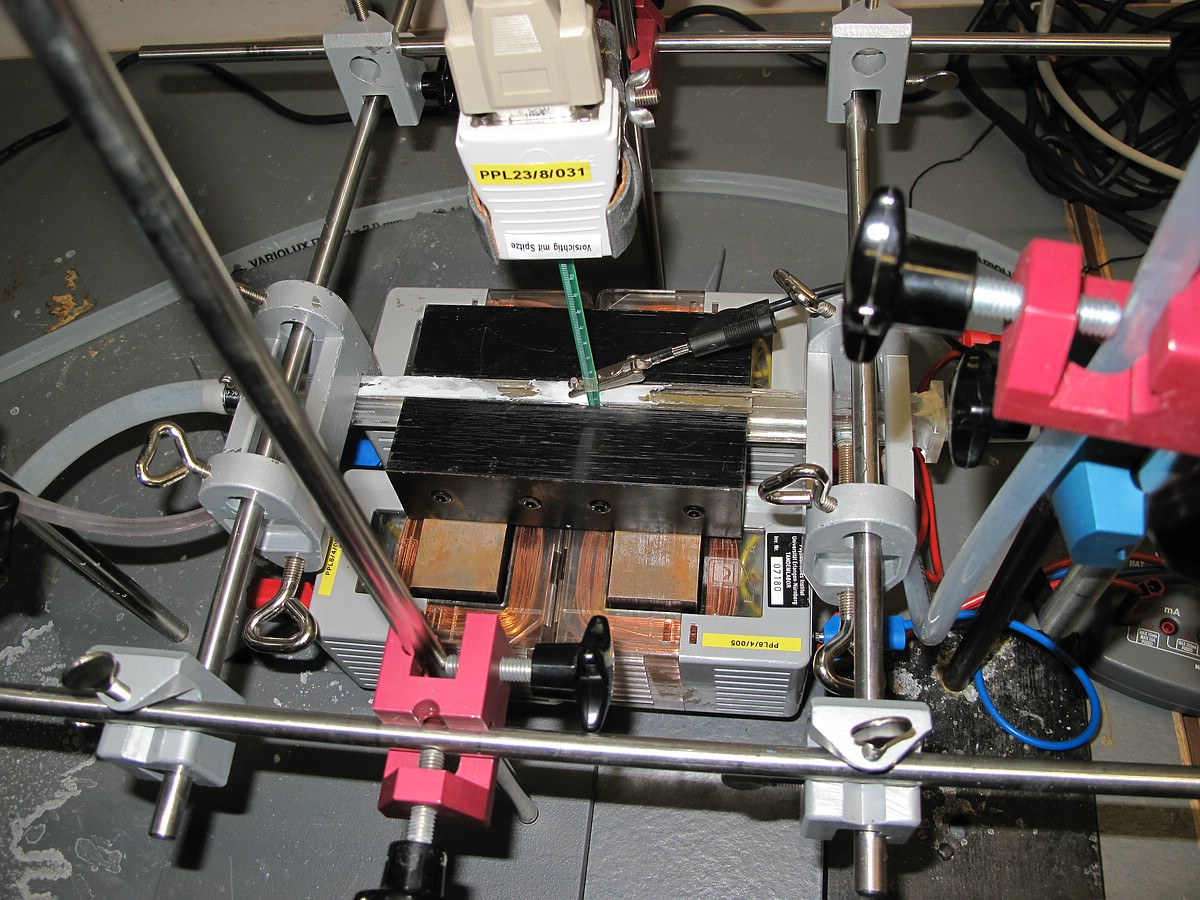
\includegraphics[width=0.8\textwidth]{images/offen.jpg}
\end{center}
\vspace{-1.5\baselineskip}
\caption{Die Magnetfeldsonde, eingeklemmt zwischen Spulenkernen und Zelle. Die Plastikt\"ute um die Spulen wurde aus optischen Gr\"unden entfernt.}
\label{offen}
\end{figure}

Zur Bestimmung des lokalen Drucks, kamen zwei d\"unne Schl\"auche als Steigrohre zum Einsatz, welche an den Seitenr\"andern der Zelle angeschlossen waren. An diesen konnte der unterschiedliche Wasserstand abgelesen werden. Um eine einheitliche Ausgangsh"ohe zu erhalten, kam als als Messbasis eine Wasserwaage zum Einsatz. Die Steigrohre wurden ebenfalls in die Konstruktion eingespannt.

\begin{figure}[ht]
\begin{center}
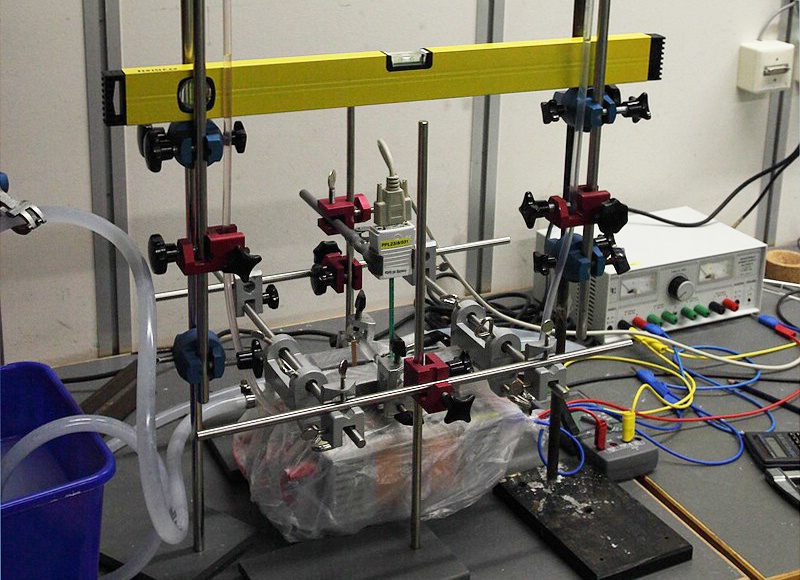
\includegraphics[width=0.8\textwidth]{images/wwaage.jpg}
\end{center}
\vspace{-1.5\baselineskip}
\caption{Der komplette Aufbau des MHD-Generators, im Eimer links befindet sich die Pumpe mit dem Wasservorrat}
\label{wwaage}
\end{figure}

Strom und Spannungsmesswerte, sowie die Magnetfeldst"arke wurden durch das Cassy Lab System mit entsprechenden Verst"arker und Anschlussboxen \"uber die Zeit aufgetragen und zur Auswertung aufgezeichnet. F\"ur die Messung des, an der Spule angelegten, Stroms im Bereich von bis zu $2A$, war der Messbereich ausreichend, es waren jedoch keine Adapter verf\"ugbar, um den an der Zelle abfallenden Strom zu verst\"arken. Daher kam auch hier wieder der Umweg \"uber einen einstellbaren Widerstand mit anschlie\"ssender Spannungsmessung zum Zuge.

\section{Messungen und Ergebnisse}

\subsection{Leitfähigkeit von Salzwasser}		%%michele
Die interessantesten Messungen gibts hier, Widerstand der Zelle

\subsection{Magnetfeld}			%%andi
Abh"angigkeit der Zellspannung vom B-Feld

\subsection{Generatorspannung und -strom}		%%basti

\subsection{Wassergeschwindigkeit und Druck}		%%evtl. 
... Wirkungsgrad gibts keinen, weil die Druckmessung zu schwierig war.

\subsection{Umkehrung des Effekts, Nutzung als Wasserpumpe}		%%david
Wird sogar als Antriebstechnik für Schiffe getestet (Magnetohydrodynamischer Antrieb bei Wikipedia)

\section{Fazit}		%%david

\newpage
\section{Autorenverzeichnis}
\begin{tabular}{|l|l|}
\hline
\emph{Autor} & \emph{Kapitel}\\
\hline
Michele Collodo & Widerstandsmessung\\
Andreas Glossner & Magnetfeldmessung\\
Karl-Christoph G\"odel & Bau der Zelle\\
Bastian Hacker & Strommessung\\
Maria Obst & Einleitung und Theorie\\
Alexander Wagner & Versuchsaufbau und Bilder\\
David Winnekens & Umkehrung des Effekts und Fazit\\
\hline
\end{tabular}

\end{document}
